\documentclass[11pt,a4paper]{article}
\usepackage[margin=1in]{geometry}
\usepackage{amsmath,amssymb}
\usepackage{tikz}
\usetikzlibrary{arrows.meta,positioning,calc,decorations.pathreplacing}
\usepackage{tcolorbox}
\usepackage{hyperref}
\usepackage{booktabs}
\usepackage{microtype}

\hypersetup{
    colorlinks=true,
    linkcolor=blue!70!black,
    citecolor=blue!70!black,
    urlcolor=blue!70!black
}

% Custom Callout Boxes matching math_tools_en / house style
\newtcolorbox{learningobj}{
    colback=blue!3!white,
    colframe=blue!60!black,
    fonttitle=\bfseries\sffamily,
    title={$\blacktriangleright$ LEARNING OBJECTIVE},
    arc=2mm,
    boxrule=1pt,
    left=4mm, right=4mm, top=3mm, bottom=3mm
}

\newtcolorbox{groundbreaking}{
    colback=teal!4!white,
    colframe=teal!60!black,
    fonttitle=\bfseries\sffamily,
    title={$\bigstar$ GROUNDBREAKING FINDING},
    arc=2mm,
    boxrule=1pt,
    left=4mm, right=4mm, top=3mm, bottom=3mm
}

\begin{document}

\section*{1.1 Intuition: The Core Divergence Between Computer Vision and Edge Voice AI}

\begin{learningobj}
Rather than treating audio processing as a black-box sequence of numerical matrices, this section guides you through the physical and mechanical machinery of sound. We deduce why voice processing diverges fundamentally from computer vision, why edge latency ruthlessly enforces an execution batch size of one ($batch=1$), and how the biological inertia of human vocal articulators dictates the real-time frame boundaries for every silicon architecture developed in this monograph.
\end{learningobj}

\subsection*{A Photograph in a Gallery vs. An Oscillating Diaphragm}

A photograph is a finished object. A sound is a physical process that has not concluded.

This single distinction governs nearly every architectural trade-off in this book. In computer vision, a digital image arrives at the processor as an intact, bounded spatial matrix. The pixels along the bottom edge exist at the exact same instant as the pixels along the top edge. Processing a second photograph does not alter the spatial reality of the first photograph; you can stack eight, sixteen, or sixty-four photographs together into a single four-dimensional tensor and launch them simultaneously through a neural network.

Grouping independent inputs in this manner is called \textbf{batching}, and the count of grouped samples represents the \textbf{batch size} ($B$). A Graphics Processing Unit (GPU)---built from thousands of lightweight arithmetic execution lanes running in lockstep under a Single Instruction, Multiple Threads (SIMT) harness---executes one massive matrix multiplication far more efficiently than it can execute sixty-four disjointed, tiny multiplications. On a desktop or cloud GPU, batching delivers an immense throughput advantage virtually for free. The only currency expended is patience---and a static photograph resting in memory has no ticking deadline.

A streaming voice signal presents the exact opposite physical reality. Acoustic data does not materialize as a complete, two-dimensional canvas; it arrives as a continuous, relentless stream of air pressure samples measured by an oscillating microphone diaphragm. To assemble a batch of eight audio frames, the processing system cannot pull future samples out of thin air. It is physically forced to hold the first audio frame captive in a waiting queue until the eighth frame has finished vibrating through the air and cleared the analog-to-digital converter.

\begin{figure}[htbp]
\centering
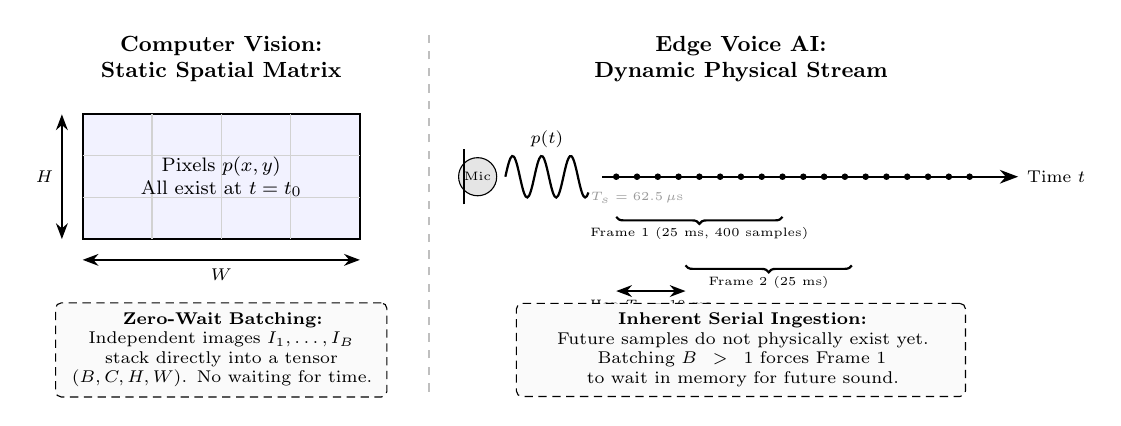
\begin{tikzpicture}[
  >=Stealth,
  scale=0.88, every node/.style={transform shape},
  ann/.style={font=\footnotesize, align=center},
  subbox/.style={draw, densely dashed, rounded corners=2pt, align=center, inner sep=4pt, font=\scriptsize, fill=gray!4}
]

% Left: Computer Vision (Static 2D Spatial Canvas)
\node[font=\bfseries\small, align=center] at (2.5, 3.8) {Computer Vision:\\Static Spatial Matrix};

\draw[thick, fill=blue!5] (0.5, 1.2) rectangle (4.5, 3.0);
\foreach \x in {1.5, 2.5, 3.5} {
  \draw[gray!35] (\x, 1.2) -- (\x, 3.0);
}
\foreach \y in {1.8, 2.4} {
  \draw[gray!35] (0.5, \y) -- (4.5, \y);
}

\node[ann] at (2.5, 2.1) {Pixels $p(x, y)$ \\ All exist at $t = t_0$};
\draw[<->, semithick] (0.2, 1.2) -- node[left, font=\scriptsize] {$H$} (0.2, 3.0);
\draw[<->, semithick] (0.5, 0.9) -- node[below, font=\scriptsize] {$W$} (4.5, 0.9);

\node[subbox, text width=4.5cm] at (2.5, -0.4) {
  \textbf{Zero-Wait Batching:}\\
  Independent images $I_1, \dots, I_B$ stack directly into a tensor $(B, C, H, W)$. No waiting for time.
};

% Vertical Separator
\draw[dashed, gray!50, thick] (5.5, -1.0) -- (5.5, 4.2);

% Right: Streaming Voice (Dynamic Temporal Wave)
\node[font=\bfseries\small, align=center] at (10.0, 3.8) {Edge Voice AI:\\Dynamic Physical Stream};

% Microphone & Sound Wave
\node[draw, circle, fill=gray!20, minimum size=0.55cm, inner sep=0pt] (mic) at (6.2, 2.1) {};
\node[font=\tiny, align=center] at (6.2, 2.1) {Mic};
\draw[thick] (6.0, 1.7) -- (6.0, 2.5);

% Incoming Acoustic Wave
\draw[thick, domain=6.6:7.8, samples=50, smooth] plot (\x, {2.1 + 0.3*sin(15*(\x-6.6)*180/3.14159)});
\node[font=\scriptsize, above] at (7.2, 2.4) {$p(t)$};

% Time Axis and Sample Ticks
\draw[thick, ->] (8.0, 2.1) -- (14.0, 2.1) node[right, font=\scriptsize] {Time $t$};
\foreach \t in {8.2, 8.5, 8.8, 9.1, 9.4, 9.7, 10.0, 10.3, 10.6, 10.9, 11.2, 11.5, 11.8, 12.1, 12.4, 12.7, 13.0, 13.3} {
  \filldraw (\t, 2.1) circle (1.1pt);
}
\node[font=\tiny, gray!80, below] at (8.5, 2.0) {$T_s = 62.5\,\mu\mathrm{s}$};

% Frames Brackets
\draw[thick, decoration={brace, mirror, raise=2pt}, decorate] (8.2, 1.6) -- node[below=3pt, font=\tiny] {Frame 1 ($25\text{ ms}$, 400 samples)} (10.6, 1.6);
\draw[thick, decoration={brace, mirror, raise=2pt}, decorate] (9.2, 0.9) -- node[below=3pt, font=\tiny] {Frame 2 ($25\text{ ms}$)} (11.6, 0.9);
\draw[<->, semithick] (8.2, 0.45) -- node[below, font=\tiny] {Hop $T_h = 10\text{ ms}$} (9.2, 0.45);

\node[subbox, text width=6.2cm] at (10.0, -0.4) {
  \textbf{Inherent Serial Ingestion:}\\
  Future samples do not physically exist yet.\\
  Batching $B > 1$ forces Frame 1 to wait in memory for future sound.
};

\end{tikzpicture}

\caption{The physical and geometric divergence between spatial computer vision and streaming edge voice. Notice that while a static 2D image matrix exists instantaneously across all spatial dimensions and permits zero-wait batching, an acoustic waveform materializes sequentially as air pressure vibrates a microphone diaphragm over physical time. This proves that an audio frame cannot be fetched from the future, making streaming ingestion inherently serial.}
\label{fig:1_1a_cv_vs_voice}
\end{figure}

\textbf{Latency} ($\tau$)---the physical elapsed time from the instant an acoustic pressure wave strikes the microphone to the instant the edge processor emits an actionable linguistic decision---is not an abstract software profiling metric. In an interactive streaming system, batching is never free: every additional item in the batch is purchased directly by sacrificing user latency.

\bigskip
\hrule
\bigskip

\subsection*{A 2-State Journey: Deducing the $batch = 1$ Mandate}

Instead of accepting ``$batch=1$'' as an arbitrary rule of thumb, let us trace the physical queue of an acoustic ingress buffer and calculate the precise arithmetic tax that batching imposes upon the listener.

\begin{itemize}
    \item \textbf{State 1 --- The Ingress Queuing Penalty:}\\
    Suppose our acoustic front end generates one analysis frame every $T_h$ seconds, where $T_h$ represents the \textbf{hop period} (the temporal stride between consecutive analysis windows). If our inference engine refuses to compute until it has assembled a batch of $B$ frames, the very first frame captured must sit completely idle in memory while frames $2, 3, \dots, B$ are being recorded:
    \[
    \Delta t_{\text{wait}} = (B - 1) \, T_h
    \]
    In this equation, $(B-1)$ represents the exact count of subsequent frame intervals that must elapse in the physical world before the batch buffer is declared full.

    \item \textbf{State 2 --- The Latency Collapse at $B = 8$:}\\
    Throughout this monograph, standard edge speech processing fixes the hop period at $T_h = 10\text{ ms}$ (a rate whose biological origin we will derive shortly). Now, suppose a system designer attempts to run an edge GPU at a modest batch size of $B = 8$ to improve SIMT hardware utilization:
    \[
    \Delta t_{\text{wait}} = (8 - 1) \times 10\text{ ms} = 70\text{ ms}
    \]
    Notice what has occurred: \textbf{$70\text{ ms}$ of pure latency has been added to the system before a single floating-point multiplication has taken place.}
    
    This $70\text{ ms}$ penalty is an unyielding arithmetic consequence of the batching policy, not an artifact of poor code or slow memory buses. In an interactive Keyword Spotting (KWS) engine or real-time voice command interface, human auditory psychology perceives any total reaction time beyond $100\text{ to }150\text{ ms}$ as unnatural, sluggish, and broken. A queuing delay of $70\text{ ms}$ instantly consumes more than half of the entire system latency budget.
\end{itemize}

\begin{figure}[htbp]
\centering
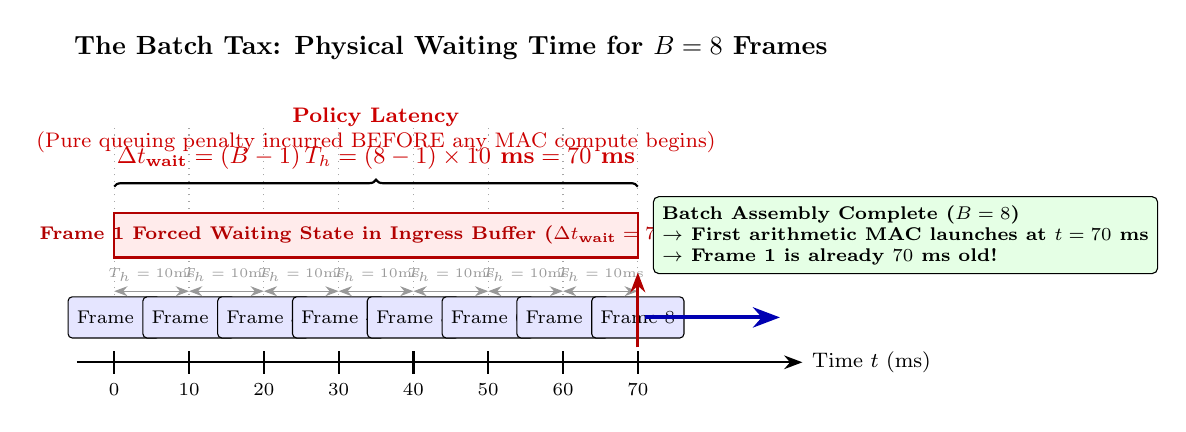
\begin{tikzpicture}[
  >=Stealth,
  scale=0.95, every node/.style={transform shape},
  framebox/.style={draw, fill=blue!10, rounded corners=1.5pt, minimum width=0.85cm, minimum height=0.55cm, font=\scriptsize, align=center},
  waitbox/.style={draw=red!70!black, fill=red!10, dashed, rounded corners=2pt, minimum height=0.6cm, font=\scriptsize, align=center},
  ann/.style={font=\footnotesize, align=center}
]

% Title
\node[font=\bfseries\normalsize, align=center] at (4.5, 4.2) {The Batch Tax: Physical Waiting Time for $B=8$ Frames};

% Time Axis
\draw[thick, ->] (-0.5, 0) -- (9.2, 0) node[right, font=\footnotesize] {Time $t$ (ms)};

% Ticks on Time Axis
\foreach \x/\val in {0/0, 1/10, 2/20, 3/30, 4/40, 5/50, 6/60, 7/70} {
  \draw[thick] (\x, 0.15) -- (\x, -0.15) node[below, font=\scriptsize] {\val};
}

% Frames arrival along time
\foreach \i/\x in {1/0, 2/1, 3/2, 4/3, 5/4, 6/5, 7/6, 8/7} {
  \node[framebox] at (\x, 0.6) {Frame \i};
  \draw[dotted, gray!70] (\x, 0.9) -- (\x, 3.2);
}

% Frame 1 Waiting Bar across 0 to 70 ms
\draw[fill=red!8, draw=red!70!black, thick] (0, 1.4) rectangle (7.0, 2.0);
\node[font=\scriptsize\bfseries, text=red!70!black] at (3.5, 1.7) {Frame 1 Forced Waiting State in Ingress Buffer ($\Delta t_{\text{wait}} = 70\text{ ms}$)};

% Hop intervals indicators
\foreach \x in {0, 1, 2, 3, 4, 5, 6} {
  \draw[<->, gray!80, thin] (\x, 0.95) -- node[above, font=\tiny] {$T_h=10\text{ms}$} (\x+1, 0.95);
}

% Top Bracket for Total Waiting Penalty
\draw[thick, decoration={brace, raise=4pt}, decorate] (0, 2.2) -- node[above=7pt, font=\small\bfseries, text=red!80!black] {
  $\Delta t_{\text{wait}} = (B - 1) \, T_h = (8 - 1) \times 10\text{ ms} = 70\text{ ms}$
} (7.0, 2.2);

\node[font=\footnotesize, align=center, text=red!80!black] at (3.5, 3.1) {
  \textbf{Policy Latency}\\(Pure queuing penalty incurred BEFORE any MAC compute begins)
};

% Trigger at 70 ms
\draw[line width=1.2pt, red!70!black, -{Stealth[length=2.5mm]}] (7.0, 0.2) -- (7.0, 1.2);
\draw[line width=1.5pt, blue!70!black, ->] (7.1, 0.6) -- (8.9, 0.6);

\node[draw, fill=green!10, rounded corners=2pt, font=\scriptsize\bfseries, align=left, anchor=west] at (7.2, 1.7) {
  \textbf{Batch Assembly Complete ($B=8$)}\\
  $\to$ First arithmetic MAC launches at $t = 70\text{ ms}$\\
  $\to$ Frame 1 is already $70\text{ ms}$ old!
};

\end{tikzpicture}

\caption{The arithmetic latency penalty imposed by input batching on an acoustic stream. Notice that Frame 1 must sit completely idle in the ingress buffer for $(B-1)T_h = 70\text{ ms}$ while subsequent frames are being physically recorded from the air. This proves that the $70\text{ ms}$ delay is policy latency dictated by the batch size $B=8$, wholly independent of processor clock speed or arithmetic multiply-accumulate (MAC) throughput.}
\label{fig:1_1b_batch_tax}
\end{figure}

\begin{groundbreaking}
An edge voice interface operating in the physical presence of a speaking human being cannot aggregate inputs over time. To preserve real-time interactivity, the system is fundamentally locked into:
\[
batch = 1
\]
The core design question for the edge hardware architect is not: \emph{``How can we compute a massive matrix batch with maximum throughput?''} \\
It is: \emph{``How can we execute ONE solitary, lightweight frame to absolute completion within a ten-millisecond budget, deterministically, repeating forever without falling behind the clock?''}
\end{groundbreaking}

\bigskip
\hrule
\bigskip

\subsection*{Three Physical Divergences: The Mechanical Constraints of Sound}

From the single reality that sound arrives sequentially in a $batch = 1$ regime, three physical consequences emerge. Each constraint directly dictates a hardware requirement in the chapters ahead.

\subsubsection*{1. Sound Possesses No Natural Boundary (The Memory State Mandate)}
A digital image is rigidly bounded by a finite pixel height $H$ and width $W$. A streaming audio waveform possesses neither: human speech continues indefinitely into the future, and an edge processor cannot observe the entire signal before beginning its work.

Because the processor cannot look ahead, it must bridge temporal continuity by preserving past context in \textbf{state}---a dedicated, tightly bounded on-chip memory that holds what the next arriving frame will need.
\begin{itemize}
    \item \emph{Hardware Bridge to Chapter 4:} This requirement transforms how we size semiconductor resources. When deploying streaming models, asking \emph{``How many multiply-accumulate (MAC) units does the chip possess?''} is secondary to the far sharper architectural question: \emph{``How many kilobits of on-chip Block RAM (BRAM) or UltraRAM (URAM) must be committed to maintain left-context state without stalling on external DRAM access?''}
\end{itemize}

\subsubsection*{2. Biological Inertia Governs Frame Overlap (The Sliding Ring Buffer Mandate)}
Why do standard acoustic pipelines enforce a $10\text{ ms}$ frame step? The answer lies in human biomechanics.

The human vocal tract---comprising the tongue, lips, velum, pharynx, and mandible---is an assembly of biological tissue with physical mass. Because these articulators possess mechanical inertia, they cannot change their physical geometry instantaneously. Consequently, human speech remains \textbf{quasi-stationary} (statistically stable in its spectral envelope) over brief intervals of $20\text{ to }30\text{ ms}$.

To capture a statistically reliable spectral snapshot, the digital front end must observe a temporal window of $25\text{ ms}$ ($400\text{ samples}$ at the standard sampling rate $f_s = 16\text{ kHz}$). However, to accurately track rapid phonetic transitions between plosives, fricatives, and vowels, the analysis window must advance in fine strides of $T_h = 10\text{ ms}$ ($160\text{ samples}$).

This biological reality creates a dramatic mechanical consequence: \textbf{consecutive frames overlap heavily}. Out of the 400 samples comprising the current analysis frame:
\[
400 - 160 = 240\text{ samples}
\]
have already been ingested, buffered, and analyzed during the preceding frame.

Copying or re-reading these 240 overlapping samples across system memory buses on every frame would squander memory bandwidth and waste dynamic power. In dedicated hardware, this overlap presents an elegant opportunity: an FPGA architecture can maintain a circular sliding buffer in local BRAM, where read and write address pointers advance smoothly along a fixed circular ring, eliminating data duplication entirely (a concept we formalize in Section 1.2 and map to FPGA silicon in Chapter 4 and Chapter 9).

\subsubsection*{3. Nature's Clock is Non-Negotiable (The Back-Pressure and Data Loss Crisis)}
A physical microphone diaphragm does not halt its mechanical oscillation simply because a downstream CPU core is servicing an operating system interrupt or experiencing a memory cache miss.

In computer vision, a congested processing queue merely delays the completion of a static frame by several milliseconds; the pixels remain intact in memory. In streaming audio, an unserviced queue causes the ingress buffer to overflow, triggering \textbf{dropped samples}. Because an acoustic waveform is an irreversible, continuous time-series, a dropped audio sample is annihilated permanently; it can never be retrieved or re-computed.

\begin{itemize}
    \item \emph{Hardware Bridge to Chapter 4 \& Chapter 8:} Chapter 4 formalizes the hardware mechanism of \textbf{back-pressure}---the structural protocol by which downstream processing units signal their readiness to upstream buffers. On an edge voice pipeline, the $10\text{ ms}$ frame budget is not a performance target or an optimization goal; it is a non-negotiable physical deadline.
\end{itemize}

\bigskip
\hrule
\bigskip

\subsection*{Redefining ``Speed'': Throughput vs. Deterministic Frame Latency}

These three mechanical constraints force a profound shift in how an engineer defines computing speed.

A computer vision accelerator is evaluated by \textbf{throughput}---the total volume of images processed per second ($\text{FPS}$) under high batch occupancy. In stark contrast, a real-time edge voice accelerator is evaluated first and foremost by \textbf{deterministic execution latency}: whether the processing engine guarantees that every single frame completes its entire extraction and classification pipeline well within its $10\text{ ms}$ physical deadline, cycle after cycle, with zero jitter. Only after this temporal contract is guaranteed does the design optimize for \textbf{energy efficiency per frame} ($\text{mJ/frame}$).

The primary reason a traditional GPU is not the natural machine for real-time edge voice is not that its arithmetic circuits are weak. Rather, its silicon area is optimized for a metric---bulk parallel throughput across wide batches---that an interactive streaming system ($batch = 1$) is physically forbidden to use.

\paragraph{Connecting to Chapter 3:} In Chapter 3, we verify this architectural bottleneck through empirical measurements on the NVIDIA Jetson Orin Nano, demonstrating the severe compute-lane starvation and power inefficiency that occur when a SIMT processor is forced to execute on single, isolated audio frames.

\bigskip
\hrule
\bigskip

\paragraph{The Unresolved Dilemma: The Streaming Ingestion Crisis}
If audio arrives as an unending, continuous stream of air pressure samples that cannot be batched without fatal latency penalties, how does an edge processor turn an infinite, continuous wave into finite mathematical packets without losing information or creating catastrophic boundary distortions?

This physical dilemma leads us directly to the mathematical machinery of the streaming preprocessing pipeline in Section 1.2.

\end{document}
